\chapter{电磁感应及其应用}\label{ch:b1:induction}

将磁铁移向线圈，线圈中便有电流流过；让磁铁
停止，电流随之中断。法拉第于 1831 年发现这一现象，此前已探索了十年，
这一事实是整个电气世界运转的基础：
每座发电站、每台变压器、每台电动机及
扬声器和麦克风，每台电磁炉和无线充电器，
都通过同一定律转换能量，即\emph{变化的}磁通量
驱动电动势。本章给出该定律及其符号约定，
阐述它所具有的两种形式：固定电路中的磁场变化，
以及在固定磁场中运动的电路；定义自感与互感，
然后讨论各类机电装置——
滑动杆、交流发电机、变压器和扬声器——
在这些装置中，同一定律将机械功率转换为电功率，
反之亦然，且决不会凭空获得能量。

\begin{omfigure}
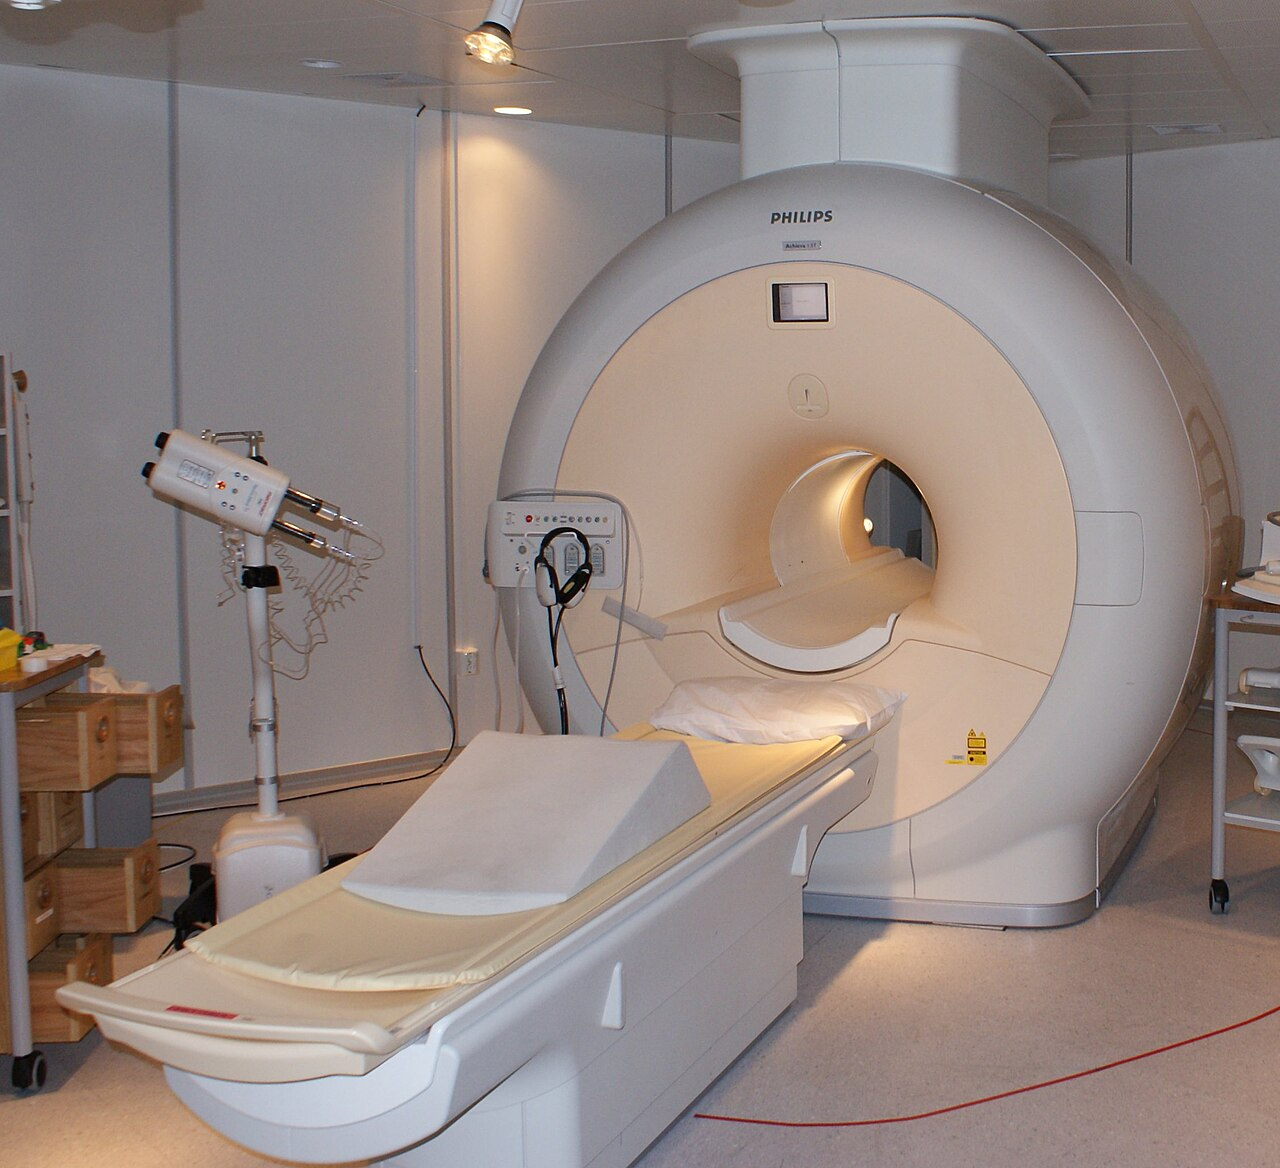
\includegraphics[width=0.50\linewidth]{images/book3/mri-scanner.jpg}

{\small 一台 MRI 扫描仪：超导螺线管在患者身上方维持 \qty{1.5}{T} 的磁场，磁场中储存着约一兆焦的磁能，而磁场内部空无一物。照片：Jan Ainali，CC~BY~3.0。}
\end{omfigure}

\section{法拉第电磁感应定律}

\begin{definition}[穿过电路的磁通量]\label{def:b1:induction:flux}
\index{磁通量}\index{韦伯}
规定闭合电路 $\Gamma$ 的绕行方向（一个走向），其所张曲面的法向量
$\vect n$ 由右手定则给出。穿过电路的\emph{磁通量}
为 $\Phi = \sum\vect B\cdot\vect n\,\dd S$，求和遍及
以 $\Gamma$ 为边界的任一曲面（单位为韦伯，$\qty{1}{Wb} = \qty{1}{T.m^2}$）——
“任一”，是因为 $\vect B$ 穿过闭合曲面的通量恒为零。
若磁场为匀强磁场，平面线圈匝数为 $N$、面积为 $S$，则 $\Phi =
NBS\cos\alpha$，其中 $\alpha$ 为 $\vect B$ 与 $\vect n$ 的夹角。
\end{definition}

\begin{theorem}[法拉第电磁感应定律]\label{thm:b1:induction:faraday}
\index{法拉第电磁感应定律}\index{感应电动势}\index{楞次定律}
只要穿过电路的磁通量发生变化，该电路中便产生
\emph{感应电动势}
\[
e = -\frac{\dd\Phi}{\dd t} ,
\]
沿电路的绕行方向计，即相当于理想电压源，
其电动势为 $e$；若电路电阻为 $R$，
则它驱动电流 $i = e/R$。式中的负号即\emph{楞次定律}：
感应电流的方向总是阻碍产生它的磁通量变化，
它自身的磁场及其所受的力，都与产生它的原因相抗衡。
\end{theorem}
\admitted

\begin{remark}[同一定律的两种形式]\label{rem:b1:induction:twofaces}
\index{诺伊曼感应}\index{洛伦兹感应}
磁通量的改变有两种原因：或是 $\vect B$ 随时间变化、穿过一个
固定电路（\emph{诺伊曼感应}：变压器、电磁炉），
或是电路在恒定磁场中运动或形变
（\emph{洛伦兹感应}：发电机、扬声器）。在第二种情形中，
电动势也可直接算出：导体元 $\dd\vect l$ 中的
载流子以 $\vect v$ 运动，受力 $q\vect v\wedge
\vect B$，它等效于电场 $\vect v\wedge\vect B$，于是
$e = \oint(\vect v\wedge\vect B)\cdot\dd\vect l$——这与
$-\dd\Phi/\dd t$ 总相符。法拉第电磁感应定律涵盖两种情形；
本科二年级分册解释了两种机制为何给出同一公式。
\end{remark}

\begin{omfigure}
\begin{tikzpicture}[font=\small, x=1cm, y=1cm, >=Stealth]
  \begin{scope}
    \draw[omThm, very thick, postaction={decorate, decoration={markings, mark=at position 0.25 with {\arrow{>}}, mark=at position 0.75 with {\arrow{>}}}}] (0,0) ellipse (1.4 and 0.5);
    \draw[omDef, thick, ->] (0,0.5) -- (0,1.7) node[right, font=\footnotesize] {$\vect n$};
    \node[omThm, font=\footnotesize] at (1.75,-0.55) {$\Gamma$};
    \foreach \x in {-0.9,-0.3,0.3,0.9} \draw[omProp, ->] (\x,-1.6) -- (\x,1.2);
    \node[omProp, font=\footnotesize] at (1.4,1.05) {$\vect B$};
    \node[font=\footnotesize] at (0,-2.2) {$\Phi = \vect B\cdot\vect n\,S > 0$};
  \end{scope}
  \begin{scope}[xshift=6.2cm]
    \draw[omThm, very thick, postaction={decorate, decoration={markings, mark=at position 0.25 with {\arrow{<}}, mark=at position 0.75 with {\arrow{<}}}}] (0,0) ellipse (1.4 and 0.5);
    \node[omThm, font=\footnotesize] at (1.75,0.6) {$i$};
    % magnet coming down
    \draw[fill=omDef!20, draw=omDef, thick] (-0.4,1.3) rectangle (0.4,2.0); \node[omDef, font=\footnotesize] at (0,1.65) {S 极};
    \draw[fill=omThm!20, draw=omThm, thick] (-0.4,2.0) rectangle (0.4,2.7); \node[omThm, font=\footnotesize] at (0,2.35) {N 极};
    \draw[very thick, ->] (0.8,2.6) -- (0.8,1.7) node[right, font=\footnotesize] {$\vect v$};
    \draw[omProp, ->] (0,1.25) -- (0,0.2) node[right, font=\footnotesize, pos=0.6] {$\vect B$（磁铁）};
    \draw[omDef, ->] (-0.6,-0.1) -- (-0.6,0.9) node[left, font=\footnotesize, pos=0.7] {$\vect B_{\text{感应}}$};
    \node[font=\footnotesize] at (0,-2.2) {磁铁靠近时：$i$ 使其受斥力};
  \end{scope}
  \begin{scope}[xshift=11.8cm]
    \draw[omThm, very thick] (-1.4,-0.5) rectangle (1.4,0.5);
    \draw[omThm, very thick] (0.5,-0.5) -- (0.5,0.5);
    \draw[omDef, very thick, ->] (0.5,0.5) -- (0.5,-0.5);
    \draw[very thick, ->] (0.6,0.75) -- (1.2,0.75) node[above, font=\footnotesize] {$\vect v$};
    \foreach \x in {-1.1,-0.6,-0.1,0.4,0.9} \node[omProp, font=\scriptsize] at (\x,0.0) {$\odot$};
    \node[omProp, font=\footnotesize] at (1.75,0.0) {$\vect B$};
    \draw[omDef, ->, thick] (0.5,0.0) -- (-0.2,0.0); \node[omDef, font=\footnotesize] at (-0.15,-0.3) {$\vect F$};
    \node[font=\footnotesize] at (0,-2.2) {滑动杆：磁通量增大，$\vect F$ 阻碍其运动};
  \end{scope}
\end{tikzpicture}

{\small 绕行方向与楞次定律。左：电路的绕行方向
决定 $\vect n$ 及 $\Phi$ 的符号。中：磁铁靠近
圆环时磁通量增大，感应电流产生的磁场与
磁铁的磁场相反，圆环受斥力。右：导体杆在导轨上滑动，
磁场方向指向读者，电路的磁通量增大，
感应电流的流向使杆所受拉普拉斯力阻碍其
运动。}
\end{omfigure}

\begin{example}[数量级]\label{ex:b1:induction:orders}
一个 $100$ 匝、面积为 \qty{10}{cm^2} 的线圈置于地磁场中，
在 \qty{0.1}{s} 内翻转：$\Delta\Phi = 2 \times 100 \times 10^{-3} \times 5 \times 10^{-5} = \qty{1e-5}{Wb}$，
$e \sim \qty{0.1}{mV}$——可用灵敏电流计测得，
正如人们曾用它测绘地磁场那样。同一线圈置于磁铁的
\qty{1}{T} 间隙中，在 \qty{0.1}{s} 内被拉出时，电动势为 \qty{1}{V}。一个变压器线圈，
匝数为 $1000$，磁场 \qty{1}{T}、频率 \qty{50}{Hz}，面积 \qty{10}{cm^2}：$e_{\max} =
1000 \times 10^{-3} \times 314 = \qty{314}{V}$——即市电。
\end{example}

\section{自感与互感}

\begin{definition}[电感]\label{def:b1:induction:inductance}
\index{自感}\index{亨利}\index{互感}
电路自身磁场穿过其自身的磁通量
与其电流成正比：$\Phi_{\text{自}} = Li$，$L > 0$ 为其\emph{自感}
（亨利，\unit{H}）。电路~1 穿过电路~2 的磁通量为
$\Phi_{1 \to 2} = Mi_1$，同理 $\Phi_{2 \to 1} = Mi_2$，$M$ 为
\emph{互感}（符号由绕行方向确定）。
于是电路~1 的总磁通量为 $\Phi_1 = L_1i_1 + Mi_2$。
\end{definition}

\begin{proposition}[电感器；螺线管]\label{prop:b1:induction:inductor}
\index{电感器}\index{磁能}\index{磁场能量密度}
电感为 $L$ 的电路中通有变化的电流时，其中产生
电动势 $e = -L\,\dd i/\dd t$：按负载约定，此即
电感器电压 $u = L\,\dd i/\dd t$，即
在\cref{ch:b1:transient-regimes}中所用的电压。其储能为 $W = \tfrac12Li^2$。
一个长螺线管，每米 $n$ 匝，长 $\ell$，截面积 $S$，
其电感为 $L = \mu_0n^2S\ell$，储能为 $\tfrac12\mu_0n^2I^2S\ell =
\dfrac{B^2}{2\mu_0}\,S\ell$：磁能储存于磁场中，其
能量密度为 $B^2/2\mu_0$，与电场能量密度 $\varepsilon_0E^2/2$ 完全对应。
\end{proposition}

\begin{proof}
由法拉第电磁感应定律，取 $\Phi = Li$，$L$ 为常量。能量方面，电感器所接收的功率为
$ui = Li\,\dd i/\dd t = \dd(\tfrac12Li^2)/\dd t$。螺线管：
内部 $B = \mu_0nI$，每匝磁通量为 $BS$，共 $n\ell$ 匝，故 $\Phi =
\mu_0n^2S\ell I$。一般形式的能量密度在本阶段不加证明地承认。
\end{proof}

\begin{example}[磁共振成像磁体]\label{ex:b1:induction:mri}
\qty{1.5}{T}，作用于约一立方米的空间：$B^2/2\mu_0 = 2.25/2.5 \times 10^{-6} =
\qty{0.9}{MJ/m^3}$——相当于汽车电池的能量，储存于真空中。
线圈电流为 \qty{500}{A} 时，$L = 2W/I^2 = \qty{7}{H}$。若
超导体突然转为有电阻的状态（即\emph{失超}），这一兆焦耳
能量在数秒内转化为热量，使数百升液
氦汽化：磁体室为此设有排放口。
\end{example}

\begin{proposition}[理想变压器]\label{prop:b1:induction:transformer}
\index{变压器}
绕在同一闭合铁芯上的两个线圈，匝数分别为 $N_1$ 和 $N_2$，
使同一磁通量 $\varphi$ 穿过每一匝，满足
\[
\frac{u_2}{u_1} = \frac{N_2}{N_1} , \qquad N_1i_1 + N_2i_2 = 0 \quad\text{（无损耗，无励磁电流）},
\]
于是 $u_2i_2 = -u_1i_1$：原边所取的功率
全部在副边输出；电压按匝数比变化，电流
则成反比。仅在电流变化时才起作用。
\end{proposition}

\begin{proof}
$u_1 = N_1\,\dd\varphi/\dd t$，$u_2 = N_2\,\dd\varphi/\dd t$（两侧均取负载约定，
绕向沿共同磁通选取）：相除即得。
电流关系由铁芯上的安培环路定理给出：其环路积分
等于 $\mu_0\mu_r$ 倍的、产生磁通量所需的总安匝数；
对于理想铁芯（$\mu_r \to \infty$），所需安匝数趋于零，
因此 $N_1i_1 + N_2i_2 = 0$。此式在本阶段不加证明地承认。
\end{proof}

\begin{omfigure}
\begin{tikzpicture}[font=\small, x=1cm, y=1cm, >=Stealth]
  % core
  \draw[omExo!60, line width=9pt] (-2,-1.5) rectangle (2,1.5);
  % primary windings
  \foreach \y in {-0.9,-0.6,...,0.9} \draw[omThm, thick] (-2.35,\y) arc[start angle=90, end angle=-90, x radius=0.18, y radius=0.15];
  \foreach \y in {-0.9,-0.6,...,0.9} \draw[omDef, thick] (2.35,\y) arc[start angle=90, end angle=270, x radius=0.18, y radius=0.15];
  \draw[omThm, thick] (-2.35,0.9) -- (-3.2,0.9) node[left, font=\footnotesize] {$u_1$}; \draw[omThm, thick] (-2.35,-1.2) -- (-3.2,-1.2);
  \draw[omDef, thick] (2.35,0.9) -- (3.2,0.9) node[right, font=\footnotesize] {$u_2$}; \draw[omDef, thick] (2.35,-1.2) -- (3.2,-1.2);
  \node[omThm, font=\footnotesize] at (-2.9,0) {$N_1$}; \node[omDef, font=\footnotesize] at (2.9,0) {$N_2$};
  \draw[omProp, thick, dashed, ->] (-1.3,-0.9) -- (-1.3,0.9) -- (1.3,0.9) -- (1.3,-0.9) -- cycle;
  \node[omProp, font=\footnotesize] at (0,0) {通量 $\varphi$};
  \node[font=\footnotesize] at (0,-2.2) {$u_2/u_1 = N_2/N_1$, \quad $N_1 i_1 = -N_2 i_2$};
  \begin{scope}[xshift=8.6cm]
    \draw[omThm, very thick] (-1.6,0) -- (1.6,0);
    \foreach \x in {-1.3,-0.9,...,1.3} \draw[omThm, thick] (\x,0) arc[start angle=180, end angle=0, x radius=0.2, y radius=0.45];
    \draw[omDef, very thick] (-1.2,-1.1) -- (1.2,-1.1);
    \foreach \x in {-0.9,-0.5,...,0.9} \draw[omDef, thick] (\x,-1.1) arc[start angle=180, end angle=0, x radius=0.2, y radius=0.35];
    \node[omThm, font=\footnotesize] at (-2.1,0.3) {$i_1$, $L_1$}; \node[omDef, font=\footnotesize] at (-1.9,-0.9) {$L_2$};
    \draw[<->, omProp] (0,0.7) -- (0,-0.9) node[midway, right, font=\footnotesize] {$M$};
    \node[font=\footnotesize] at (0,-2.2) {$\Phi_1 = L_1 i_1 + M i_2$};
  \end{scope}
\end{tikzpicture}

{\small 左：变压器——两线圈绕于闭合铁芯上，共享
同一磁通；电压与匝数成正比，电流
成反比。右：空气中的两个耦合线圈及其
互感 $M$；线圈自身的磁通量为 $Li$。}
\end{omfigure}

\section{运动导体：发电机与电动机}

\begin{proposition}[滑动导体棒]\label{prop:b1:induction:rails}
\index{拉普拉斯导轨}\index{机电转换}
长为 $\ell$ 的导体棒以速率 $v$ 在两根导轨上滑动，两导轨由
电阻 $R$ 闭合，置于与平面垂直的匀强磁场 $B$ 中。它是
产生电动势 $e = B\ell v$，驱动电流 $i = B\ell v/R$，并受到
拉普拉斯力 $F = B\ell i = B^2\ell^2v/R$，\emph{阻碍}其运动。
推动它所需的机械功率 $Fv$ 等于
所耗散的电功率 $ei = Ri^2$：导体棒即为发电机。若改由
电源 $E$ 供电，则它是电动机：电流 $(E - B\ell v)/R$ 推动它
直至反电动势 $B\ell v$ 与 $E$ 平衡，此时的空载速率为 $E/B\ell$。
\end{proposition}

\begin{proof}
磁通量为 $B\ell x$，$e = -B\ell\dot x$，取使 $\vect n$
与 $\vect B$ 同向的绕向；电流所受的拉普拉斯力 $i\vect\ell\wedge\vect B$
在此绕向下，其方向与 $\vect v$ 相反（见\cref{thm:b1:induction:faraday}，
楞次定律）。将电路方程 $e = Ri$ 乘以 $i$，将
力学方程乘以 $v$，得 $Fv = B\ell iv = ei$。机电
功率 $ei$ 与拉普拉斯功率 $-Fv$ 始终相反——此即
机电转换的规律。
\end{proof}

\begin{proposition}[旋转线圈：交流发电机]\label{prop:b1:induction:alternator}
\index{交流发电机}
匝数为 $N$、面积为 $S$ 的线圈，绕一根轴以 $\omega$ 转动，
该轴垂直于均匀磁场 $B$，其磁通量为 $\Phi = NBS\cos\omega t$，且
\[
e = NBS\omega\sin\omega t :
\]
正弦电动势，振幅为 $NBS\omega$，频率等于转动频率。
接入电阻 $R$ 时，其平均功率为 $(NBS\omega)^2/2R$，
该功率由维持其转动的力矩提供，此力矩须克服
线圈自身电流所受的拉普拉斯力偶 $-\vect m\wedge\vect B$。
\end{proposition}

\begin{proof}
对磁通求导；$\langle\sin^2\rangle = \tfrac12$。力偶
由\cref{thm:b1:magnetostatics:dipoleinfield}给出，其中 $m = Ni S$；
其平均功率 $\langle\Gamma\omega\rangle$ 与 $\langle ei\rangle$ 相等，
由与导体棒情形相同的计算可得。
\end{proof}

\begin{omfigure}
\begin{tikzpicture}[font=\small, x=1cm, y=1cm, >=Stealth]
  \begin{scope}
    \draw[omThm, very thick] (-1.8,-1.0) -- (1.8,-1.0); \draw[omThm, very thick] (-1.8,1.0) -- (1.8,1.0);
    \draw[omThm, very thick] (-1.8,-1.0) -- (-1.8,1.0);
    \draw[omDef, very thick] (0.8,-1.0) -- (0.8,1.0);
    \draw[omDef, very thick, ->] (0.8,-0.2) -- (0.8,0.3) node[right, font=\footnotesize] {$i$};
    \draw[omProp, thick, ->] (0.8,0) -- (0.05,0) node[above, font=\footnotesize, pos=0.5] {$\vect F$};
    \draw[very thick, ->] (1.0,1.25) -- (1.7,1.25) node[right, font=\footnotesize] {$\vect v$};
    \foreach \x in {-1.4,-0.9,-0.4,0.1,1.3} \foreach \y in {-0.5,0.5} \node[omProp, font=\scriptsize] at (\x,\y) {$\odot$};
    \draw[fill=white] (-1.95,-0.35) rectangle (-1.65,0.35); \node[font=\footnotesize] at (-2.45,0) {$R$};
    \node[font=\footnotesize] at (0,-1.6) {$e = B\ell v$, \; $F = B^2\ell^2 v/R$};
  \end{scope}
  \begin{scope}[xshift=6.5cm]
    \draw[omThm, very thick, rotate=30] (-1.2,-0.6) rectangle (1.2,0.6);
    \draw[dashed] (0,-1.6) -- (0,1.6); \node[font=\footnotesize] at (0,1.85) {轴};
    \foreach \y in {-1.2,-0.6,0,0.6,1.2} \draw[omProp, ->] (-2.2,\y) -- (2.2,\y);
    \node[omProp, font=\footnotesize] at (2.0,1.45) {$\vect B$};
    \draw[->, very thick] (0,0) -- (120:1.0) node[above left, font=\footnotesize] {$\vect n$};
    \draw (0.6,0) arc[start angle=0, end angle=120, radius=0.6] node[midway, above right, font=\footnotesize] {$\omega t$};
    \node[font=\footnotesize] at (0,-2.0) {$\Phi = NBS\cos\omega t$, \; $e = NBS\omega\sin\omega t$};
  \end{scope}
\end{tikzpicture}\hfill
\begin{tikzpicture}
\begin{axis}[omaxis, axis x line=middle, axis y line=left, width=4.3cm, height=3.8cm,
    xlabel={$t$}, ylabel={$e$}, xmin=0, xmax=6.6, ymin=-1.3, ymax=1.3, xtick=\empty, ytick=\empty, samples=80,
    xlabel style={at={(axis description cs:1.0,0.55)}, anchor=west}]
  \addplot[omDef, thick, domain=0:6.28] {sin(deg(x))};
\end{axis}
\end{tikzpicture}

{\small 左图：滑动导体棒作为发电机——电动势 $B\ell v$，电流
经 $R$ 流通，拉普拉斯力使导体棒减速；推力的功率
全部转化为电阻器的热量。中图与右图：交流发电机的旋转线圈
及其正弦电动势。}
\end{omfigure}

\begin{example}[涡流]\label{ex:b1:induction:eddy}
\index{涡流}
大块导体在非均匀磁场中运动，或静置于变化的磁场中，
其内无数闭合路径上的磁通量随之变化：
\emph{涡流}在其中环流，使其发热，并依楞次定律
使其减速。磁铁落入铜管后缓慢下落；卡车与过山车的
制动器便利用此原理（无接触、无磨损、不会失灵——
但静止时无制动作用）；电磁炉借助同样的电流加热锅体，
频率为 \qty{25}{kHz}；变压器铁芯
做成叠片，正是为了减小涡流。
\end{example}

\section{扬声器：耦合系统}

\begin{proposition}[线圈在辐向磁场中的机电耦合]\label{prop:b1:induction:loudspeaker}
\index{扬声器}\index{麦克风}
总导线长为 $\ell$ 的线圈置于辐向磁场 $B$ 中，使
导线每一段都与 $\vect B$ 垂直；线圈沿其轴线
以速率 $v$ 运动，通有电流 $i$。此时它受沿轴向的拉普拉斯力
$F = B\ell i$，并为反电动势 $e = -B\ell v$ 的来源（取受电器约定：电压 $B\ell v$）。
质量为 $m$、劲度系数为 $k$ 的悬挂，机械阻尼为 $h$，
由电压 $u$ 供电，
线圈的电阻为 $R$、电感为 $L$：
\[
u = Ri + L\frac{\dd i}{\dd t} + B\ell v , \qquad
m\frac{\dd v}{\dd t} = -kx - hv + B\ell i .
\]
分别乘以 $i$ 与 $v$ 后相加：电功率 $ui$
等于焦耳热损耗 $Ri^2$，加上储能的增长
$\tfrac12Li^2 + \tfrac12mv^2 + \tfrac12kx^2$，再加上机械损耗
$hv^2$（其中包括声音）；转换项 $B\ell iv$ 在两方程中
相互抵消。反过来运行（给定运动、读出 $u$），同一装置即为
动态\emph{麦克风}。
\end{proposition}

\begin{proof}
每段导线所受拉普拉斯力 $i\,\dd\vect l\wedge\vect B$ 均沿轴向，
方向相同；电动势由 $(\vect v\wedge\vect B)\cdot\dd\vect l$ 沿导线
求和得到。能量平衡即两方程
按上述方式乘后相加。
\end{proof}

\begin{omfigure}
\begin{tikzpicture}[font=\small, x=1cm, y=1cm, >=Stealth]
  % magnet structure (cross-section)
  \draw[fill=omExo!30, draw=omExo, thick] (-3.0,-1.2) rectangle (-0.6,1.2);
  \draw[fill=omExo!30, draw=omExo, thick] (-0.6,-0.35) rectangle (1.6,0.35);
  \draw[fill=omExo!30, draw=omExo, thick] (-0.6,0.85) rectangle (1.6,1.2);
  \draw[fill=omExo!30, draw=omExo, thick] (-0.6,-1.2) rectangle (1.6,-0.85);
  \node[omExo, font=\footnotesize] at (-1.8,0) {磁铁};
  % coil in the gaps
  \foreach \x in {0.9,1.05,1.2,1.35} {\fill[omThm] (\x,0.6) circle (1.6pt); \fill[omThm] (\x,-0.6) circle (1.6pt);}
  \node[omThm, font=\footnotesize] at (1.1,1.55) {音圈};
  % radial field arrows in the gaps
  \foreach \x in {0.3,0.55} {\draw[omProp, ->] (\x,0.4) -- (\x,0.8); \draw[omProp, ->] (\x,-0.4) -- (\x,-0.8);}
  \node[omProp, font=\footnotesize] at (-0.2,0.6) {$\vect B$};
  % cone
  \draw[thick] (1.6,0.6) -- (3.4,2.2); \draw[thick] (1.6,-0.6) -- (3.4,-2.2);
  \draw[thick] (1.6,0.6) -- (1.6,-0.6);
  \node[font=\footnotesize] at (2.9,-0.95) {纸盆，$m$};
  \draw[thick, decorate, decoration={coil, aspect=0.6, segment length=3pt, amplitude=2pt}] (3.4,2.2) -- (3.4,2.9); \draw[thick] (3.0,2.9) -- (3.8,2.9);
  \draw[thick, decorate, decoration={coil, aspect=0.6, segment length=3pt, amplitude=2pt}] (3.4,-2.2) -- (3.4,-2.9); \draw[thick] (3.0,-2.9) -- (3.8,-2.9);
  \node[font=\footnotesize] at (3.4,3.25) {悬挂 $k$、$h$};
  \draw[omDef, very thick, ->] (1.6,0) -- (2.6,0);
  \node[omDef, font=\footnotesize, anchor=south west] at (1.75,0.08) {$F = B\ell i$};
  \draw[very thick, ->] (4.6,0.5) -- (5.6,0.5) node[right, font=\footnotesize] {$v$};
  \node[font=\footnotesize] at (5.3,-1.7) {$u = Ri + L\frac{\dd i}{\dd t} + B\ell v$};
\end{tikzpicture}

{\small 动圈式扬声器剖面示意：音圈置于
磁铁的环形间隙中，间隙内磁场沿径向，因此
无论位置如何，通电线圈都受到沿轴向的力；它所驱动的纸盆
由刚度较大且带阻尼的悬挂支撑；线圈的运动在电路中
产生反电动势 $B\ell v$。}
\end{omfigure}

\begin{remark}[为何耦合会产生阻尼]\label{rem:b1:induction:damping}
低频（$L\omega \ll R$）下，$i \approx (u - B\ell v)/R$，受力
为 $B\ell u/R - (B^2\ell^2/R)\,v$：电路
为机械运动增加了阻尼 $B^2\ell^2/R$。接在放大器上的
扬声器（输出电阻低）阻尼很大——纸盆
信号一停即停止振动——同样的耦合也使话筒
能够从声音中获取能量（见\cref{pb:b1:induction:1}）。
\end{remark}

\section{练习}

\begin{exercise}[$\star$]\label{exo:b1:induction:1}
线圈共 $100$ 匝，面积 \qty{10}{cm^2}，置于均匀磁场 \qty{0.20}{T} 中，磁场与
线圈法线成 \qty{30}{\degree}。求磁通量；若磁场在
\qty{10}{ms} 内撤去，求平均感应电动势；若在 \qty{1}{ms} 内撤去，
则再求一次，并用楞次定律判断感应电流相对原磁场的方向。
\end{exercise}

\begin{exercise}[$\star$]\label{exo:b1:induction:2}
一根长 \qty{20}{cm} 的导体棒以 \qty{2.0}{m/s} 的速度在导轨上滑动，
导轨另一端接有 \qty{0.10}{\ohm} 的电阻，磁场为 \qty{0.50}{T}，求感应电动势、电流、拉普拉斯力、
推动者需施加的力、机械功率和电功率。
\end{exercise}

\begin{exercise}[$\star$]\label{exo:b1:induction:3}
螺线管每米 \qty{1000}{turns/m}，长 \qty{20}{cm}，截面积 \qty{4.0}{cm^2}：
求自感；电流为 \qty{5.0}{A} 时的能量；与 \qty{1.0}{\ohm}
电阻串联时的时间常数；内部磁场及能量密度，并核对是否等于 $B^2/2\mu_0$。
\end{exercise}

\begin{exercise}[$\star$]\label{exo:b1:induction:4}
一台变压器由 \qty{230}{V} 降为 \qty{12}{V}。求匝数比；
副线圈为 $50$ 匝时原线圈的匝数；副线圈
输出 \qty{2.0}{A} 电流时原线圈中的电流。它为什么不能接在汽车电池上工作？
\end{exercise}

\begin{exercise}[$\star\star$]\label{exo:b1:induction:5}
应用楞次定律：给出各情形中感应电流的方向，以及
受力的方向——(a) 北极沿轴线靠近一个圆环；
(b) 圆环置于逐渐增强的磁场中；(c) 圆环落到磁铁上；
(d) 磁铁穿过一根长铜管下落。对于 (d)，
请用能量观点解释它为何以较小的恒定速率下落。
\end{exercise}

\begin{exercise}[$\star\star$]\label{exo:b1:induction:6}
交流发电机：$N = 200$，$S = \qty{20}{cm^2}$，$B = \qty{0.10}{T}$，频率 \qty{50}{Hz}。
求电动势的峰值与有效值；接入 \qty{10}{\ohm} 电阻时的峰值电流与峰值力矩；平均
电功率；将其与平均机械功率比较，并与
电动势为零时刻的瞬时力矩比较。
\end{exercise}

\begin{exercise}[$\star\star$]\label{exo:b1:induction:7}
\emph{电磁制动。}一个边长 $a = \qty{10}{cm}$ 的方形线框，
电阻 $R = \qty{1.0}{m\ohm}$，质量 \qty{1.0}{kg}，从
磁场为 $B = \qty{1.0}{T}$ 的匀强磁场区域，以速率 $v$ 离开
（此时仍有一边在磁场中）。求感应电动势、电流与制动力；列出运动方程并求时间
常数；求从 \qty{1.0}{m/s} 出发直至停止所经过的距离；
动能去了哪里？
\end{exercise}

\begin{exercise}[$\star\star$]\label{exo:b1:induction:8}
一个小线圈（$N_2 = 50$ 匝，横截面积 \qty{2.0}{cm^2}）置于
一根长螺线管（$n_1 = \qty{2000}{m^{-1}}$）内部，二者轴线平行。求互感；
求线圈中的电动势：当螺线管电流以
\qty{100}{A/s} 的速率变化时，以及电流为 $\qty{1.0}{A}$、频率为 \qty{10}{kHz} 时的情形。$M$
是否与哪一个线圈通电有关？
\end{exercise}

\begin{exercise}[$\star\star$]\label{exo:b1:induction:9}
磁场能量：$B = \qty{1.5}{T}$ 充满 \qty{1.0}{m^3}，如同 MRI
磁体中的情形。求能量；$I = \qty{500}{A}$ 时的电感；该能量能将
质量为 \qty{1}{t} 的汽车举高多少；失超时能使多少体积的液氦沸腾
（每升 \qty{2.6}{kJ}）。求地球磁场
（\qty{5e-5}{T}）在 \qty{50}{m^3} 的房间内的能量。
\end{exercise}

\begin{exercise}[$\star\star\star$]\label{exo:b1:induction:10}
\emph{作为电动机的导轨。}\cref{exo:b1:induction:2} 中的导体棒（质量 $m$，
无摩擦）与电源 $E$ 通过电阻 $R$ 相连。
(a) 列出电学与力学方程，并证明 $m\,\dd v/\dd t = B\ell(E -
B\ell v)/R$。(b) 求终端速率与时间常数。(c) 功率平衡：
电源功率 $=$ 焦耳热 $+$ 机械功率；效率作为
$v$ 的函数。(d) 数值计算：$E = \qty{2.0}{V}$，$m = \qty{50}{g}$，其余同
\cref{exo:b1:induction:2}。(e) 一个导轨炮使质量为 \qty{10}{g} 的
弹丸在 \qty{1}{T} 的磁场中，以 \qty{1}{MA} 的电流在 \qty{5}{m} 内加速，求出口速率
（取数量级）。
\end{exercise}

\begin{exercise}[$\star\star\star$]\label{exo:b1:induction:11}
\emph{法拉第圆盘。}一个半径为 $R$ 的铜盘以角速度 $\omega$
绕其轴旋转，置于沿轴向的匀强磁场 $B$ 中；电刷分别接触圆心
与盘缘。(a) 求圆心与盘缘之间的电动势：沿一条半径对 $(\vect v\wedge
\vect B)\cdot\dd\vect l$ 求和，得 $e = \tfrac12B\omega R^2$。(b) 数值计算：
$R = \qty{10}{cm}$，\qty{3000}{rpm}，\qty{1.0}{T}。(c) 为何它是低电压、
大电流装置？求接入 \qty{1}{m\ohm} 电阻时的电流，以及
制动力矩。(d) 对回路应用法拉第定律，重新得到 $e$：
回路为电刷–半径–盘缘–电刷，哪一个磁通量在变化？
\end{exercise}

\begin{exercise}[$\star\star\star$]\label{exo:b1:induction:12}
\emph{电磁炉。}玻璃面板下的线圈通有 $i_1 =
I_1\cos\omega t$，其中 $I_1 = \qty{30}{A}$，频率 \qty{25}{kHz}；锅底
相当于一匝电阻为 $R_p = \qty{10}{m\ohm}$ 的线圈，
并以 $M = \qty{1.0}{\micro H}$ 耦合（忽略锅底这一匝的自感）。(a) 求锅底中感应电动势的
峰值。(b) 求锅底中的电流及平均耗散功率。
(c) 为什么要用高频？为什么热量会出现在
锅底而不在玻璃中？(d) 锅底中的电流反作用于线圈：
在线圈中感应出的电动势（峰值），以及发电机必须额外
提供的功率——验证其等于 (b) 中的结果。
\end{exercise}

\begin{omfigure}

\includegraphics[width=0.58\linewidth]{images/book3/ai/b3-29-bicycle-dynamo.jpg}

{\small 瓶式发电机：车轮带动线圈内的磁铁转动，穿过线圈的磁通量随之变化，灯便亮起——自行车上的法拉第电磁感应定律。}
\end{omfigure}

\section{问题：自行车发电机与扬声器}

\begin{problem}[{周末问题——两个机电转换器的拆解：
一台能自我调节的发电机，以及
其放大器兼作制动器的扬声器}]
\label{pb:b1:induction:1}

\medskip
\noindent\textbf{第一部分——自行车发电机。}
一个匝数 $N = 300$、面积 $S = \qty{3.0}{cm^2}$ 的线圈，
置于均匀磁场 $B = \qty{0.30}{T}$ 中；其转轴上装有一只
半径为 $r = \qty{1.0}{cm}$ 的滚轮，紧压在轮胎上，
因此线圈以 $\omega = v/r$ 转动，$v$ 为自行车速度。线圈电阻 $r_c = \qty{4.0}{\ohm}$，
自感 $L = \qty{20}{mH}$；灯泡为电阻 $R = \qty{12}{\ohm}$ 的负载。
\begin{enumerate}
  \item 穿过线圈的磁通量与感应电动势随时间的函数关系；
        幅值与频率（$v = \qty{18}{km/h}$）。
  \item 先忽略 $L$，求 \qty{18}{km/h} 时灯泡中的有效值电流与功率；
        “\qty{6}{V}、\qty{3}{W}”的灯泡能否正常工作？
  \item 求骑车人提供给发电机的平均机械功率，
        以及轮胎上相应的作用力（与
        约 \qty{2}{N} 的滚动摩擦力比较）。
  \item 用楞次定律解释发电机为何产生阻碍，以及
        灯泡“免费”发光为何与能量守恒并不矛盾。
  \item 计入 $L$：求电路的复阻抗；证明电流幅值
        为 $I = NBS\omega/\sqrt{(R + r_c)^2 + L^2\omega^2}$，
        并说明其在高速时趋于饱和；求其极限值，以及
        电流达到该极限值 $70\%$ 时的速度。
  \item 若不计自感，下坡时车速为 \qty{54}{km/h}，灯泡能获得多少功率？
        计入自感后又如何？
  \item 求车速为 \qty{9}{km/h} 与 \qty{36}{km/h} 时的电流及灯泡功率，
        并评论其自我调节作用。
  \item 实际发电机是让磁铁在固定线圈内转动。分析是否因此改变？
        它消除了什么实际问题？
  \item 自行车在红灯前停下时，灯泡会怎样？
        现代车灯如何解决这一问题？
\end{enumerate}

\medskip
\noindent\textbf{第二部分——扬声器。}
音圈：导线长 $\ell = \qty{5.0}{m}$，置于径向磁场 $B =
\qty{1.0}{T}$ 中，电阻 $R = \qty{8.0}{\ohm}$，自感 $L = \qty{0.50}{mH}$；
运动质量（线圈与纸盆）$m = \qty{10}{g}$；悬挂劲度
$k = \qty{1000}{N/m}$，机械阻尼 $h = \qty{1.0}{N.s/m}$。正弦稳态，
取复振幅。
\begin{enumerate}[resume]
  \item 求电流为 $i$ 时线圈所受的力，以及速度为 $v$ 时的反电动势；
        两者均需推导，并注明正负号。
  \item 写出电路方程与力学方程。
  \item 消去 $i$，证明
        $\underline v = \dfrac{B\ell\,\underline u}{(R + jL\omega)(jm\omega + h + k/j\omega) + B^2\ell^2}$。
  \item 在 $L\omega \ll R$ 的频率下，证明耦合作用
        相当于附加的机械阻尼 $B^2\ell^2/R$；求其数值，以及纸盆的
        共振频率，以及计入与不计电学阻尼时的
        品质因数。
  \item 放大器输出幅值为 \qty{1.0}{A}、频率为 \qty{1}{kHz} 的电流 $i$：
        求纸盆在质量控制区的力、加速度、位移与速度幅值；
        比较反电动势幅值与
        $Ri$。
  \item 同一电流在共振频率下：求速度幅值
        （阻尼控制区）与反电动势，并加以评论。
  \item 求 \qty{1}{kHz} 时的电功率；求消耗于 $h$ 中的机械功率
        （视为声音与悬挂损耗）；求效率。
  \item 为何声压与纸盆的加速度成正比（在本阶段不加证明地承认）？
        这一关系是否解释了质量控制的纸盆
        在共振以上给出平坦响应？
  \item 为何磁场必须是径向的？高音单元为何做得很小？
  \item 画出放大器所见阻抗 $\underline u/\underline i$ 的模随
        \qty{10}{Hz} 至 \qty{10}{kHz} 变化的示意图：标出低频处的值，
        共振处的值（使用阻尼控制区的速度），
        以及 \qty{10}{kHz} 处的值。
\end{enumerate}

\medskip
\noindent\textbf{第三部分——逆向运行与参考书目。}
\begin{enumerate}[resume]
  \item 同一装置用作传声器：声音使纸盆以
        $v = \qty{1.0}{mm/s}$ 运动；求开路电压。
  \item 接入负载 $R_L = \qty{600}{\ohm}$：求电流及作用于纸盆的制动力；
        证明传声器从声音中获取功率，其等效阻尼为
        $B^2\ell^2/(R + R_L)$。
  \item 线圈绕在铝制圆筒（骨架）上，
        相当于一匝长 \qty{0.10}{m}、电阻为 \qty{1.0}{m\ohm} 的闭合线圈：
        分析其附加的阻尼；说明骨架为何要开槽。
  \item 轻敲接线柱开路的扬声器的纸盆，再轻敲接线柱短路的扬声器的纸盆：
        哪一个的余音更长，
        为什么？
  \item 写出扬声器在稳态下一个周期内的能量平衡式，
        并逐项说明各项。
  \item 总结：对每种装置，列出所用的定律，以及
        值得记住的两个数值。
\end{enumerate}
\end{problem}
